% **************************************************************************************************************
% A Classic Thesis Style
% An Homage to The Elements of Typographic Style
%
% Copyright (C) 2018 André Miede and Ivo Pletikosić
%
% If you like the style then I would appreciate a postcard. My address
% can be found in the file ClassicThesis.pdf. A collection of the
% postcards I received so far is available online at
% http://postcards.miede.de
%
% License:
% This program is free software; you can redistribute it and/or modify
% it under the terms of the GNU General Public License as published by
% the Free Software Foundation; either version 2 of the License, or
% (at your option) any later version.
%
% This program is distributed in the hope that it will be useful,
% but WITHOUT ANY WARRANTY; without even the implied warranty of
% MERCHANTABILITY or FITNESS FOR A PARTICULAR PURPOSE.  See the
% GNU General Public License for more details.
%
% You should have received a copy of the GNU General Public License
% along with this program; see the file COPYING.  If not, write to
% the Free Software Foundation, Inc., 59 Temple Place - Suite 330,
% Boston, MA 02111-1307, USA.
%
% PLEASE SEE ALSO THE AUTHORS' NOTE REGARDING THIS LICENSE
% IN THE DOCUMENTATION (ClassicThesis.pdf --> Chapter 1 / Chapter01.tex)
% **************************************************************************************************************

% Before `documentclass` as recommended by pdfx package
% !TeX root = ./Thesis.tex

\newcommand{\myTitle}{iOS CommCenter Fuzzing}
\newcommand{\myDegree}{Master Thesis}
%\newcommand{\myDegreePhD}{Doktor-Ingenieur (Dr.-Ing.)}
\newcommand{\myName}{Kristian Zeitzschel}
%\newcommand{\myBirthDate}{\formatdate{15}{4}{1997}} % only for PhD thesis
%\newcommand{\myBirthPlace}{Darmstadt, Deutschland} % only for PhD thesis
%\newcommand{\myNationality}{German} % only for PhD thesis
\newcommand{\myProf}{Prof. Dr.-Ing. Matthias Hollick}
%\newcommand{\myOtherProf}{Put name here} % only for PhD thesis
\newcommand{\mySupervisor}{Dr. Jiska Classen}
\newcommand{\myThesiscode}{SEEMOO-MSC-$0000$} % You will get this from our secretary
\newcommand{\myFaculty}{Department of Computer Science}
\newcommand{\myFacultyDE}{Fachbereich Informatik}
\newcommand{\myDepartment}{Secure Mobile Networking Lab}
\newcommand{\myDepartmentDE}{Fachgebiet Sichere Mobile Netze}
\newcommand{\myUni}{\protect{Technische Universität Darmstadt}}
\newcommand{\myUniKennziffer}{D17}
\newcommand{\myLocation}{Darmstadt}
\newcommand{\myTime}{\formatdate{01}{01}{1337}} % hand-in date of the thesis
%\newcommand{\myYearPublication}{1337} % year of publication (only for PhD thesis)
%\newcommand{\myYearPresent}{1337} % year of disputation (only for PhD thesis)
%\newcommand{\myTimePresent}{\formatdate{01}{01}{\myYearPresent}} % date of disputation (only for PhD thesis)
\newcommand{\myVersion}{0.1}
%\newcommand{\myURN}{urn:nbn:de:tuda-tuprints-83253} % only for PhD thesis
\newcommand{\myAbstract}{Short summary of the contents} % at the very end, put your "clean" abstract here
\begin{filecontents*}{\jobname.xmpdata}
\Title{\myTitle}
\Author{\myName}
\Copyright{Copyright \copyright\ \myYearPublication "\myName"}
%\Keywords{Wi-Fi\sep Reverse Engineering\sep macOS}
\Subject{\myAbstract} % Make sure to update your abstract!
\end{filecontents*}

\RequirePackage{silence} % :-\
    \WarningFilter{scrreprt}{Usage of package `titlesec'}
    %\WarningFilter{scrreprt}{Activating an ugly workaround}
    \WarningFilter{titlesec}{Non standard sectioning command detected}
\documentclass[ twoside,openright,titlepage,numbers=noenddot,%1headlines,
                headinclude,footinclude,cleardoublepage=empty,abstract=on,
                BCOR=5mm,paper=a4,fontsize=11pt
                ]{scrreprt}

%********************************************************************
% PDF/A for TUbama
%*******************************************************
\PassOptionsToPackage{dvipsnames}{xcolor}
\usepackage[a-1b]{pdfx}

%********************************************************************
% Note: Make all your adjustments in here
%*******************************************************
\usepackage{etoolbox}
\newtoggle{adrianstyle}
%\toggletrue{adrianstyle} % uncomment this line to have smaller margins
\PassOptionsToPackage{adrianstyle=\iftoggle{adrianstyle}{true}{false}}{classicthesis}
\newtoggle{parts}
%\toggletrue{parts} % uncomment to use parts (for long theses only!)
\newtoggle{phd}
%\toggletrue{phd} % uncomment to write a full-blown PhD thesis (with parts, author references, etc.)
\iftoggle{phd}{\toggletrue{parts}}{}

% !TeX root = ./Thesis.tex

% ****************************************************************************************************
% classicthesis-config.tex
% formerly known as loadpackages.sty, classicthesis-ldpkg.sty, and classicthesis-preamble.sty
% Use it at the beginning of your ClassicThesis.tex, or as a LaTeX Preamble
% in your ClassicThesis.{tex,lyx} with % !TeX root = ./Thesis.tex

% ****************************************************************************************************
% classicthesis-config.tex
% formerly known as loadpackages.sty, classicthesis-ldpkg.sty, and classicthesis-preamble.sty
% Use it at the beginning of your ClassicThesis.tex, or as a LaTeX Preamble
% in your ClassicThesis.{tex,lyx} with % !TeX root = ./Thesis.tex

% ****************************************************************************************************
% classicthesis-config.tex
% formerly known as loadpackages.sty, classicthesis-ldpkg.sty, and classicthesis-preamble.sty
% Use it at the beginning of your ClassicThesis.tex, or as a LaTeX Preamble
% in your ClassicThesis.{tex,lyx} with \input{classicthesis-config}
% ****************************************************************************************************
% If you like the classicthesis, then I would appreciate a postcard.
% My address can be found in the file ClassicThesis.pdf. A collection
% of the postcards I received so far is available online at
% http://postcards.miede.de
% ****************************************************************************************************


% ****************************************************************************************************
% 0. Set the encoding of your files. UTF-8 is the only sensible encoding nowadays. If you can't read
% äöüßáéçèê∂åëæƒÏ€ then change the encoding setting in your editor, not the line below. If your editor
% does not support utf8 use another editor!
% ****************************************************************************************************
\PassOptionsToPackage{utf8}{inputenc}
  \usepackage{inputenc}

\PassOptionsToPackage{T1}{fontenc} % T2A for cyrillics
  \usepackage{fontenc}


% ****************************************************************************************************
% 1. Configure classicthesis for your needs here, e.g., remove "drafting" below
% in order to deactivate the time-stamp on the pages
% (see ClassicThesis.pdf for more information):
% ****************************************************************************************************
\PassOptionsToPackage{
  drafting=false,    % print version information on the bottom of the pages
  tocaligned=false, % the left column of the toc will be aligned (no indentation)
  dottedtoc=true,  % page numbers in ToC flushed right
  eulerchapternumbers=true, % use AMS Euler for chapter font (otherwise Palatino)
  linedheaders=false,       % chaper headers will have line above and beneath
  floatperchapter=false,     % numbering per chapter for all floats (i.e., Figure 1.1)
  eulermath=true,  % use awesome Euler fonts for mathematical formulae (only with pdfLaTeX)
  beramono=true,    % toggle a nice monospaced font (w/ bold)
  palatino=true,    % deactivate standard font for loading another one, see the last section at the end of this file for suggestions
  style=classicthesis % classicthesis, arsclassica
}{classicthesis}


% ****************************************************************************************************
% 2. Personal data and user ad-hoc commands (insert your own data here)
% ****************************************************************************************************
% MOVED TO `classicthesis-personal-info.tex`

% ********************************************************************
% Setup, finetuning, and useful commands
% ********************************************************************
\providecommand{\mLyX}{L\kern-.1667em\lower.25em\hbox{Y}\kern-.125emX\@}
% ****************************************************************************************************


% ****************************************************************************************************
% 3. Loading some handy packages
% ****************************************************************************************************
% ********************************************************************
% Packages with options that might require adjustments
% ********************************************************************
\PassOptionsToPackage{ngerman,american}{babel} % change this to your language(s), main language last
% Spanish languages need extra options in order to work with this template
%\PassOptionsToPackage{spanish,es-lcroman}{babel}
    \usepackage{babel}

\PassOptionsToPackage{autostyle=true}{csquotes}
    \usepackage{csquotes}
\PassOptionsToPackage{%
  backend=biber,bibencoding=utf8, %instead of bibtex
  %backend=bibtex8,bibencoding=ascii,%
  language=auto,%
  style=numeric-comp,%
  %style=authoryear-comp, % Author 1999, 2010
  %bibstyle=authoryear,dashed=false, % dashed: substitute rep. author with ---
  sorting=nyt, % name, year, title
  maxbibnames=10, % default: 3, et al.
  %backref=true,%
  defernumbers=true, % enable so split references (author's publications) have continuous numbers
  natbib=true % natbib compatibility mode (\citep and \citet still work)
}{biblatex}
    \usepackage{biblatex}

\PassOptionsToPackage{fleqn}{amsmath}       % math environments and more by the AMS
  \usepackage{amsmath}

% ********************************************************************
% General useful packages
% ********************************************************************
\usepackage{graphicx} %
\usepackage{scrhack} % fix warnings when using KOMA with listings package
\usepackage{xspace} % to get the spacing after macros right
\PassOptionsToPackage{style=long,nopostdot,acronym,shortcuts,nonumberlist,nolist}{glossaries}
  \usepackage{glossaries}
\makeglossary

% ****************************************************************************************************
%\usepackage{pgfplots} % External TikZ/PGF support (thanks to Andreas Nautsch)
%\usetikzlibrary{external}
%\tikzexternalize[mode=list and make, prefix=ext-tikz/]
% ****************************************************************************************************


% ****************************************************************************************************
% 4. Setup floats: tables, (sub)figures, and captions
% ****************************************************************************************************
\usepackage{tabularx} % better tables
  \setlength{\extrarowheight}{3pt} % increase table row height
\newcommand{\tableheadline}[1]{\multicolumn{1}{@{}l@{}}{\spacedlowsmallcaps{#1}}}
\newcommand{\myfloatalign}{\centering} % to be used with each float for alignment
\usepackage{subcaption}
\usepackage{caption}
% ****************************************************************************************************


% ****************************************************************************************************
% 5. Setup code listings
% ****************************************************************************************************
\usepackage{listings}
\lstset{
  % color scheme follows template
  commentstyle=\color{CTsemi},
  keywordstyle={\color{CTtitle}},
  stringstyle=\color{CTcitation},
  basicstyle=\ttfamily\lst@ifdisplaystyle\small\fi, % use normal font size in \lstinline
  emphstyle={\color{CTlink}},
  tabsize=2,
  showstringspaces=false,
  captionpos=b, % caption below listing
  %belowcaptionskip=.75\baselineskip
  breaklines=true,
  frame=tb,
  numberstyle=\scriptsize,%\tiny
  numbers=left,%none,%
  stepnumber=1,
  numbersep=8pt,
}
% ****************************************************************************************************




% ****************************************************************************************************
% 6. Last calls before the bar closes
% ****************************************************************************************************
% ********************************************************************
% Her Majesty herself
% ********************************************************************
\usepackage{classicthesis}


% ********************************************************************
% Fine-tune hyperreferences (hyperref should be called last)
% ********************************************************************
\hypersetup{%
  %draft, % hyperref's draft mode, for printing see below
  colorlinks=true, linktocpage=true,
  %pdfstartpage=3, pdfstartview=FitV,%
  % uncomment the following line if you want to have black links (e.g., for printing)
  %colorlinks=false, linktocpage=false, pdfstartpage=3, pdfstartview=FitV, pdfborder={0 0 0},%
  breaklinks=true, pageanchor=true,%
  %pdfpagemode=UseNone, %
  % pdfpagemode=UseOutlines,%
  plainpages=false, bookmarksnumbered, bookmarksopen=true, bookmarksopenlevel=1,%
  hypertexnames=true,
  %pdfhighlight=/O,
  %nesting=true,%frenchlinks,%
  urlcolor=CTurl, linkcolor=CTlink, citecolor=CTcitation, %pagecolor=RoyalBlue,%
  %urlcolor=Black, linkcolor=Black, citecolor=Black, %pagecolor=Black,%
  %pdftitle={\myTitle{}},%
  %pdfauthor={\textcopyright\ \myName{}, \myUni{}, \myFaculty{}},%
  %pdfsubject={\myAbstract},%
  %pdfkeywords={},%
  %pdfcreator={pdfLaTeX},%
  %pdfproducer={LaTeX with hyperref and classicthesis}%
}


% ********************************************************************
% Setup autoreferences (hyperref and babel)
% ********************************************************************
% There are some issues regarding autorefnames
% http://www.tex.ac.uk/cgi-bin/texfaq2html?label=latexwords
% you have to redefine the macros for the
% language you use, e.g., american, ngerman
% (as chosen when loading babel/AtBeginDocument)
% ********************************************************************
\makeatletter
\@ifpackageloaded{babel}%
  {%
    \addto\extrasamerican{%
      \renewcommand*{\figureautorefname}{Figure}%
      \renewcommand*{\tableautorefname}{Table}%
      \renewcommand*{\partautorefname}{Part}%
      \renewcommand*{\chapterautorefname}{Chapter}%
      \renewcommand*{\sectionautorefname}{Section}%
      \renewcommand*{\subsectionautorefname}{Section}%
      \renewcommand*{\subsubsectionautorefname}{Section}%
    }%
    \addto\extrasngerman{%
      \renewcommand*{\paragraphautorefname}{Absatz}%
      \renewcommand*{\subparagraphautorefname}{Unterabsatz}%
      \renewcommand*{\footnoteautorefname}{Fu\"snote}%
      \renewcommand*{\FancyVerbLineautorefname}{Zeile}%
      \renewcommand*{\theoremautorefname}{Theorem}%
      \renewcommand*{\appendixautorefname}{Anhang}%
      \renewcommand*{\equationautorefname}{Gleichung}%
      \renewcommand*{\itemautorefname}{Punkt}%
    }%
      % Fix to getting autorefs for subfigures right (thanks to Belinda Vogt for changing the definition)
      \providecommand{\subfigureautorefname}{\figureautorefname}%
    }{\relax}
\makeatother


% ********************************************************************
% Development Stuff
% ********************************************************************
\listfiles
%\PassOptionsToPackage{l2tabu,orthodox,abort}{nag}
%  \usepackage{nag}
%\PassOptionsToPackage{warning, all}{onlyamsmath}
%  \usepackage{onlyamsmath}


% ****************************************************************************************************
% 7. Further adjustments (experimental)
% ****************************************************************************************************
% ********************************************************************
% Changing the text area
% ********************************************************************
%\areaset[current]{312pt}{761pt} % 686 (factor 2.2) + 33 head + 42 head \the\footskip
%\setlength{\marginparwidth}{7em}%
%\setlength{\marginparsep}{2em}%

% ********************************************************************
% Using different fonts
% ********************************************************************
%\usepackage[oldstylenums]{kpfonts} % oldstyle notextcomp
% \usepackage[osf]{libertine}
%\usepackage[light,condensed,math]{iwona}
%\renewcommand{\sfdefault}{iwona}
%\usepackage{lmodern} % <-- no osf support :-(
%\usepackage{cfr-lm} %
%\usepackage[urw-garamond]{mathdesign} <-- no osf support :-(
%\usepackage[default,osfigures]{opensans} % scale=0.95
%\usepackage[sfdefault]{FiraSans}
% \usepackage[opticals,mathlf]{MinionPro} % onlytext
% ********************************************************************
%\usepackage[largesc,osf]{newpxtext}
%\linespread{1.05} % a bit more for Palatino
% Used to fix these:
% https://bitbucket.org/amiede/classicthesis/issues/139/italics-in-pallatino-capitals-chapter
% https://bitbucket.org/amiede/classicthesis/issues/45/problema-testatine-su-classicthesis-style
% ********************************************************************
% ****************************************************************************************************

% ****************************************************************************************************
% If you like the classicthesis, then I would appreciate a postcard.
% My address can be found in the file ClassicThesis.pdf. A collection
% of the postcards I received so far is available online at
% http://postcards.miede.de
% ****************************************************************************************************


% ****************************************************************************************************
% 0. Set the encoding of your files. UTF-8 is the only sensible encoding nowadays. If you can't read
% äöüßáéçèê∂åëæƒÏ€ then change the encoding setting in your editor, not the line below. If your editor
% does not support utf8 use another editor!
% ****************************************************************************************************
\PassOptionsToPackage{utf8}{inputenc}
  \usepackage{inputenc}

\PassOptionsToPackage{T1}{fontenc} % T2A for cyrillics
  \usepackage{fontenc}


% ****************************************************************************************************
% 1. Configure classicthesis for your needs here, e.g., remove "drafting" below
% in order to deactivate the time-stamp on the pages
% (see ClassicThesis.pdf for more information):
% ****************************************************************************************************
\PassOptionsToPackage{
  drafting=false,    % print version information on the bottom of the pages
  tocaligned=false, % the left column of the toc will be aligned (no indentation)
  dottedtoc=true,  % page numbers in ToC flushed right
  eulerchapternumbers=true, % use AMS Euler for chapter font (otherwise Palatino)
  linedheaders=false,       % chaper headers will have line above and beneath
  floatperchapter=false,     % numbering per chapter for all floats (i.e., Figure 1.1)
  eulermath=true,  % use awesome Euler fonts for mathematical formulae (only with pdfLaTeX)
  beramono=true,    % toggle a nice monospaced font (w/ bold)
  palatino=true,    % deactivate standard font for loading another one, see the last section at the end of this file for suggestions
  style=classicthesis % classicthesis, arsclassica
}{classicthesis}


% ****************************************************************************************************
% 2. Personal data and user ad-hoc commands (insert your own data here)
% ****************************************************************************************************
% MOVED TO `classicthesis-personal-info.tex`

% ********************************************************************
% Setup, finetuning, and useful commands
% ********************************************************************
\providecommand{\mLyX}{L\kern-.1667em\lower.25em\hbox{Y}\kern-.125emX\@}
% ****************************************************************************************************


% ****************************************************************************************************
% 3. Loading some handy packages
% ****************************************************************************************************
% ********************************************************************
% Packages with options that might require adjustments
% ********************************************************************
\PassOptionsToPackage{ngerman,american}{babel} % change this to your language(s), main language last
% Spanish languages need extra options in order to work with this template
%\PassOptionsToPackage{spanish,es-lcroman}{babel}
    \usepackage{babel}

\PassOptionsToPackage{autostyle=true}{csquotes}
    \usepackage{csquotes}
\PassOptionsToPackage{%
  backend=biber,bibencoding=utf8, %instead of bibtex
  %backend=bibtex8,bibencoding=ascii,%
  language=auto,%
  style=numeric-comp,%
  %style=authoryear-comp, % Author 1999, 2010
  %bibstyle=authoryear,dashed=false, % dashed: substitute rep. author with ---
  sorting=nyt, % name, year, title
  maxbibnames=10, % default: 3, et al.
  %backref=true,%
  defernumbers=true, % enable so split references (author's publications) have continuous numbers
  natbib=true % natbib compatibility mode (\citep and \citet still work)
}{biblatex}
    \usepackage{biblatex}

\PassOptionsToPackage{fleqn}{amsmath}       % math environments and more by the AMS
  \usepackage{amsmath}

% ********************************************************************
% General useful packages
% ********************************************************************
\usepackage{graphicx} %
\usepackage{scrhack} % fix warnings when using KOMA with listings package
\usepackage{xspace} % to get the spacing after macros right
\PassOptionsToPackage{style=long,nopostdot,acronym,shortcuts,nonumberlist,nolist}{glossaries}
  \usepackage{glossaries}
\makeglossary

% ****************************************************************************************************
%\usepackage{pgfplots} % External TikZ/PGF support (thanks to Andreas Nautsch)
%\usetikzlibrary{external}
%\tikzexternalize[mode=list and make, prefix=ext-tikz/]
% ****************************************************************************************************


% ****************************************************************************************************
% 4. Setup floats: tables, (sub)figures, and captions
% ****************************************************************************************************
\usepackage{tabularx} % better tables
  \setlength{\extrarowheight}{3pt} % increase table row height
\newcommand{\tableheadline}[1]{\multicolumn{1}{@{}l@{}}{\spacedlowsmallcaps{#1}}}
\newcommand{\myfloatalign}{\centering} % to be used with each float for alignment
\usepackage{subcaption}
\usepackage{caption}
% ****************************************************************************************************


% ****************************************************************************************************
% 5. Setup code listings
% ****************************************************************************************************
\usepackage{listings}
\lstset{
  % color scheme follows template
  commentstyle=\color{CTsemi},
  keywordstyle={\color{CTtitle}},
  stringstyle=\color{CTcitation},
  basicstyle=\ttfamily\lst@ifdisplaystyle\small\fi, % use normal font size in \lstinline
  emphstyle={\color{CTlink}},
  tabsize=2,
  showstringspaces=false,
  captionpos=b, % caption below listing
  %belowcaptionskip=.75\baselineskip
  breaklines=true,
  frame=tb,
  numberstyle=\scriptsize,%\tiny
  numbers=left,%none,%
  stepnumber=1,
  numbersep=8pt,
}
% ****************************************************************************************************




% ****************************************************************************************************
% 6. Last calls before the bar closes
% ****************************************************************************************************
% ********************************************************************
% Her Majesty herself
% ********************************************************************
\usepackage{classicthesis}


% ********************************************************************
% Fine-tune hyperreferences (hyperref should be called last)
% ********************************************************************
\hypersetup{%
  %draft, % hyperref's draft mode, for printing see below
  colorlinks=true, linktocpage=true,
  %pdfstartpage=3, pdfstartview=FitV,%
  % uncomment the following line if you want to have black links (e.g., for printing)
  %colorlinks=false, linktocpage=false, pdfstartpage=3, pdfstartview=FitV, pdfborder={0 0 0},%
  breaklinks=true, pageanchor=true,%
  %pdfpagemode=UseNone, %
  % pdfpagemode=UseOutlines,%
  plainpages=false, bookmarksnumbered, bookmarksopen=true, bookmarksopenlevel=1,%
  hypertexnames=true,
  %pdfhighlight=/O,
  %nesting=true,%frenchlinks,%
  urlcolor=CTurl, linkcolor=CTlink, citecolor=CTcitation, %pagecolor=RoyalBlue,%
  %urlcolor=Black, linkcolor=Black, citecolor=Black, %pagecolor=Black,%
  %pdftitle={\myTitle{}},%
  %pdfauthor={\textcopyright\ \myName{}, \myUni{}, \myFaculty{}},%
  %pdfsubject={\myAbstract},%
  %pdfkeywords={},%
  %pdfcreator={pdfLaTeX},%
  %pdfproducer={LaTeX with hyperref and classicthesis}%
}


% ********************************************************************
% Setup autoreferences (hyperref and babel)
% ********************************************************************
% There are some issues regarding autorefnames
% http://www.tex.ac.uk/cgi-bin/texfaq2html?label=latexwords
% you have to redefine the macros for the
% language you use, e.g., american, ngerman
% (as chosen when loading babel/AtBeginDocument)
% ********************************************************************
\makeatletter
\@ifpackageloaded{babel}%
  {%
    \addto\extrasamerican{%
      \renewcommand*{\figureautorefname}{Figure}%
      \renewcommand*{\tableautorefname}{Table}%
      \renewcommand*{\partautorefname}{Part}%
      \renewcommand*{\chapterautorefname}{Chapter}%
      \renewcommand*{\sectionautorefname}{Section}%
      \renewcommand*{\subsectionautorefname}{Section}%
      \renewcommand*{\subsubsectionautorefname}{Section}%
    }%
    \addto\extrasngerman{%
      \renewcommand*{\paragraphautorefname}{Absatz}%
      \renewcommand*{\subparagraphautorefname}{Unterabsatz}%
      \renewcommand*{\footnoteautorefname}{Fu\"snote}%
      \renewcommand*{\FancyVerbLineautorefname}{Zeile}%
      \renewcommand*{\theoremautorefname}{Theorem}%
      \renewcommand*{\appendixautorefname}{Anhang}%
      \renewcommand*{\equationautorefname}{Gleichung}%
      \renewcommand*{\itemautorefname}{Punkt}%
    }%
      % Fix to getting autorefs for subfigures right (thanks to Belinda Vogt for changing the definition)
      \providecommand{\subfigureautorefname}{\figureautorefname}%
    }{\relax}
\makeatother


% ********************************************************************
% Development Stuff
% ********************************************************************
\listfiles
%\PassOptionsToPackage{l2tabu,orthodox,abort}{nag}
%  \usepackage{nag}
%\PassOptionsToPackage{warning, all}{onlyamsmath}
%  \usepackage{onlyamsmath}


% ****************************************************************************************************
% 7. Further adjustments (experimental)
% ****************************************************************************************************
% ********************************************************************
% Changing the text area
% ********************************************************************
%\areaset[current]{312pt}{761pt} % 686 (factor 2.2) + 33 head + 42 head \the\footskip
%\setlength{\marginparwidth}{7em}%
%\setlength{\marginparsep}{2em}%

% ********************************************************************
% Using different fonts
% ********************************************************************
%\usepackage[oldstylenums]{kpfonts} % oldstyle notextcomp
% \usepackage[osf]{libertine}
%\usepackage[light,condensed,math]{iwona}
%\renewcommand{\sfdefault}{iwona}
%\usepackage{lmodern} % <-- no osf support :-(
%\usepackage{cfr-lm} %
%\usepackage[urw-garamond]{mathdesign} <-- no osf support :-(
%\usepackage[default,osfigures]{opensans} % scale=0.95
%\usepackage[sfdefault]{FiraSans}
% \usepackage[opticals,mathlf]{MinionPro} % onlytext
% ********************************************************************
%\usepackage[largesc,osf]{newpxtext}
%\linespread{1.05} % a bit more for Palatino
% Used to fix these:
% https://bitbucket.org/amiede/classicthesis/issues/139/italics-in-pallatino-capitals-chapter
% https://bitbucket.org/amiede/classicthesis/issues/45/problema-testatine-su-classicthesis-style
% ********************************************************************
% ****************************************************************************************************

% ****************************************************************************************************
% If you like the classicthesis, then I would appreciate a postcard.
% My address can be found in the file ClassicThesis.pdf. A collection
% of the postcards I received so far is available online at
% http://postcards.miede.de
% ****************************************************************************************************


% ****************************************************************************************************
% 0. Set the encoding of your files. UTF-8 is the only sensible encoding nowadays. If you can't read
% äöüßáéçèê∂åëæƒÏ€ then change the encoding setting in your editor, not the line below. If your editor
% does not support utf8 use another editor!
% ****************************************************************************************************
\PassOptionsToPackage{utf8}{inputenc}
  \usepackage{inputenc}

\PassOptionsToPackage{T1}{fontenc} % T2A for cyrillics
  \usepackage{fontenc}


% ****************************************************************************************************
% 1. Configure classicthesis for your needs here, e.g., remove "drafting" below
% in order to deactivate the time-stamp on the pages
% (see ClassicThesis.pdf for more information):
% ****************************************************************************************************
\PassOptionsToPackage{
  drafting=false,    % print version information on the bottom of the pages
  tocaligned=false, % the left column of the toc will be aligned (no indentation)
  dottedtoc=true,  % page numbers in ToC flushed right
  eulerchapternumbers=true, % use AMS Euler for chapter font (otherwise Palatino)
  linedheaders=false,       % chaper headers will have line above and beneath
  floatperchapter=false,     % numbering per chapter for all floats (i.e., Figure 1.1)
  eulermath=true,  % use awesome Euler fonts for mathematical formulae (only with pdfLaTeX)
  beramono=true,    % toggle a nice monospaced font (w/ bold)
  palatino=true,    % deactivate standard font for loading another one, see the last section at the end of this file for suggestions
  style=classicthesis % classicthesis, arsclassica
}{classicthesis}


% ****************************************************************************************************
% 2. Personal data and user ad-hoc commands (insert your own data here)
% ****************************************************************************************************
% MOVED TO `classicthesis-personal-info.tex`

% ********************************************************************
% Setup, finetuning, and useful commands
% ********************************************************************
\providecommand{\mLyX}{L\kern-.1667em\lower.25em\hbox{Y}\kern-.125emX\@}
% ****************************************************************************************************


% ****************************************************************************************************
% 3. Loading some handy packages
% ****************************************************************************************************
% ********************************************************************
% Packages with options that might require adjustments
% ********************************************************************
\PassOptionsToPackage{ngerman,american}{babel} % change this to your language(s), main language last
% Spanish languages need extra options in order to work with this template
%\PassOptionsToPackage{spanish,es-lcroman}{babel}
    \usepackage{babel}

\PassOptionsToPackage{autostyle=true}{csquotes}
    \usepackage{csquotes}
\PassOptionsToPackage{%
  backend=biber,bibencoding=utf8, %instead of bibtex
  %backend=bibtex8,bibencoding=ascii,%
  language=auto,%
  style=numeric-comp,%
  %style=authoryear-comp, % Author 1999, 2010
  %bibstyle=authoryear,dashed=false, % dashed: substitute rep. author with ---
  sorting=nyt, % name, year, title
  maxbibnames=10, % default: 3, et al.
  %backref=true,%
  defernumbers=true, % enable so split references (author's publications) have continuous numbers
  natbib=true % natbib compatibility mode (\citep and \citet still work)
}{biblatex}
    \usepackage{biblatex}

\PassOptionsToPackage{fleqn}{amsmath}       % math environments and more by the AMS
  \usepackage{amsmath}

% ********************************************************************
% General useful packages
% ********************************************************************
\usepackage{graphicx} %
\usepackage{scrhack} % fix warnings when using KOMA with listings package
\usepackage{xspace} % to get the spacing after macros right
\PassOptionsToPackage{style=long,nopostdot,acronym,shortcuts,nonumberlist,nolist}{glossaries}
  \usepackage{glossaries}
\makeglossary

% ****************************************************************************************************
%\usepackage{pgfplots} % External TikZ/PGF support (thanks to Andreas Nautsch)
%\usetikzlibrary{external}
%\tikzexternalize[mode=list and make, prefix=ext-tikz/]
% ****************************************************************************************************


% ****************************************************************************************************
% 4. Setup floats: tables, (sub)figures, and captions
% ****************************************************************************************************
\usepackage{tabularx} % better tables
  \setlength{\extrarowheight}{3pt} % increase table row height
\newcommand{\tableheadline}[1]{\multicolumn{1}{@{}l@{}}{\spacedlowsmallcaps{#1}}}
\newcommand{\myfloatalign}{\centering} % to be used with each float for alignment
\usepackage{subcaption}
\usepackage{caption}
% ****************************************************************************************************


% ****************************************************************************************************
% 5. Setup code listings
% ****************************************************************************************************
\usepackage{listings}
\lstset{
  % color scheme follows template
  commentstyle=\color{CTsemi},
  keywordstyle={\color{CTtitle}},
  stringstyle=\color{CTcitation},
  basicstyle=\ttfamily\lst@ifdisplaystyle\small\fi, % use normal font size in \lstinline
  emphstyle={\color{CTlink}},
  tabsize=2,
  showstringspaces=false,
  captionpos=b, % caption below listing
  %belowcaptionskip=.75\baselineskip
  breaklines=true,
  frame=tb,
  numberstyle=\scriptsize,%\tiny
  numbers=left,%none,%
  stepnumber=1,
  numbersep=8pt,
}
% ****************************************************************************************************




% ****************************************************************************************************
% 6. Last calls before the bar closes
% ****************************************************************************************************
% ********************************************************************
% Her Majesty herself
% ********************************************************************
\usepackage{classicthesis}


% ********************************************************************
% Fine-tune hyperreferences (hyperref should be called last)
% ********************************************************************
\hypersetup{%
  %draft, % hyperref's draft mode, for printing see below
  colorlinks=true, linktocpage=true,
  %pdfstartpage=3, pdfstartview=FitV,%
  % uncomment the following line if you want to have black links (e.g., for printing)
  %colorlinks=false, linktocpage=false, pdfstartpage=3, pdfstartview=FitV, pdfborder={0 0 0},%
  breaklinks=true, pageanchor=true,%
  %pdfpagemode=UseNone, %
  % pdfpagemode=UseOutlines,%
  plainpages=false, bookmarksnumbered, bookmarksopen=true, bookmarksopenlevel=1,%
  hypertexnames=true,
  %pdfhighlight=/O,
  %nesting=true,%frenchlinks,%
  urlcolor=CTurl, linkcolor=CTlink, citecolor=CTcitation, %pagecolor=RoyalBlue,%
  %urlcolor=Black, linkcolor=Black, citecolor=Black, %pagecolor=Black,%
  %pdftitle={\myTitle{}},%
  %pdfauthor={\textcopyright\ \myName{}, \myUni{}, \myFaculty{}},%
  %pdfsubject={\myAbstract},%
  %pdfkeywords={},%
  %pdfcreator={pdfLaTeX},%
  %pdfproducer={LaTeX with hyperref and classicthesis}%
}


% ********************************************************************
% Setup autoreferences (hyperref and babel)
% ********************************************************************
% There are some issues regarding autorefnames
% http://www.tex.ac.uk/cgi-bin/texfaq2html?label=latexwords
% you have to redefine the macros for the
% language you use, e.g., american, ngerman
% (as chosen when loading babel/AtBeginDocument)
% ********************************************************************
\makeatletter
\@ifpackageloaded{babel}%
  {%
    \addto\extrasamerican{%
      \renewcommand*{\figureautorefname}{Figure}%
      \renewcommand*{\tableautorefname}{Table}%
      \renewcommand*{\partautorefname}{Part}%
      \renewcommand*{\chapterautorefname}{Chapter}%
      \renewcommand*{\sectionautorefname}{Section}%
      \renewcommand*{\subsectionautorefname}{Section}%
      \renewcommand*{\subsubsectionautorefname}{Section}%
    }%
    \addto\extrasngerman{%
      \renewcommand*{\paragraphautorefname}{Absatz}%
      \renewcommand*{\subparagraphautorefname}{Unterabsatz}%
      \renewcommand*{\footnoteautorefname}{Fu\"snote}%
      \renewcommand*{\FancyVerbLineautorefname}{Zeile}%
      \renewcommand*{\theoremautorefname}{Theorem}%
      \renewcommand*{\appendixautorefname}{Anhang}%
      \renewcommand*{\equationautorefname}{Gleichung}%
      \renewcommand*{\itemautorefname}{Punkt}%
    }%
      % Fix to getting autorefs for subfigures right (thanks to Belinda Vogt for changing the definition)
      \providecommand{\subfigureautorefname}{\figureautorefname}%
    }{\relax}
\makeatother


% ********************************************************************
% Development Stuff
% ********************************************************************
\listfiles
%\PassOptionsToPackage{l2tabu,orthodox,abort}{nag}
%  \usepackage{nag}
%\PassOptionsToPackage{warning, all}{onlyamsmath}
%  \usepackage{onlyamsmath}


% ****************************************************************************************************
% 7. Further adjustments (experimental)
% ****************************************************************************************************
% ********************************************************************
% Changing the text area
% ********************************************************************
%\areaset[current]{312pt}{761pt} % 686 (factor 2.2) + 33 head + 42 head \the\footskip
%\setlength{\marginparwidth}{7em}%
%\setlength{\marginparsep}{2em}%

% ********************************************************************
% Using different fonts
% ********************************************************************
%\usepackage[oldstylenums]{kpfonts} % oldstyle notextcomp
% \usepackage[osf]{libertine}
%\usepackage[light,condensed,math]{iwona}
%\renewcommand{\sfdefault}{iwona}
%\usepackage{lmodern} % <-- no osf support :-(
%\usepackage{cfr-lm} %
%\usepackage[urw-garamond]{mathdesign} <-- no osf support :-(
%\usepackage[default,osfigures]{opensans} % scale=0.95
%\usepackage[sfdefault]{FiraSans}
% \usepackage[opticals,mathlf]{MinionPro} % onlytext
% ********************************************************************
%\usepackage[largesc,osf]{newpxtext}
%\linespread{1.05} % a bit more for Palatino
% Used to fix these:
% https://bitbucket.org/amiede/classicthesis/issues/139/italics-in-pallatino-capitals-chapter
% https://bitbucket.org/amiede/classicthesis/issues/45/problema-testatine-su-classicthesis-style
% ********************************************************************
% ****************************************************************************************************

% !TeX root = ./Thesis.tex

\PassOptionsToPackage{capitalize,noabbrev,ngerman,english}{cleveref} % need to pass languages explicitly
	\usepackage{cleveref}

\usepackage{datetime} % for formating submission date

\usepackage{lipsum} % for template text

% include Git commit hash when drafting
\makeatletter
\ifthenelse{\boolean{ct@drafting}}{
	\usepackage{gitinfo2}
	\renewcommand{\PrelimText}{\footnotesize[\,\today\ at \thistime\ -- version \myVersion{} -- git \gitAbbrevHash\,]}
}{}
\makeatother

\iftoggle{phd}{
	\usepackage[LabelsAligned]{currvita} % nice cv style
}{}

% to enable wide text/floats taking the space of margin notes (435pt instead of 336pt)
% note that this changes the \linewidth (not \textwidth), so follow this example
% to include a wide figure:
%\begin{figure}
%\begin{wide}
%	
\includegraphics[width=\linewidth]{gfx/logos/tud_logo}
%	\caption{Athene logo of TU Darmstadt.}
%\end{wide}
%\end{figure}
\usepackage[strict]{changepage}
\newenvironment{wide}%
{\begin{adjustwidth*}{}{-\marginparsep-\marginparwidth}}%
{\end{adjustwidth*}}

% TikZ/PGFPlots
\usepackage{tikz}
\usepackage{pgfplots}
\pgfplotsset{compat=newest}
\usetikzlibrary{dsp,chains}
\usetikzlibrary{positioning}
%\DeclareMathAlphabet{\mathpzc}{OT1}{pzc}{m}{it}
%\newcommand{\z}{\mathpzc{z}}
% To cache tikz pictures you have to run pdflatex with -shell-escape or --enable-write18
\ifnum\pdfshellescape=1
\usepgfplotslibrary{external}
\tikzexternalize[prefix=gfxcompiled/]
\fi

% Lengths for matlab2tikz
\newlength\figureheight
\newlength\figurewidth 


%********************************************************************
% Bibliographies
%*******************************************************
\addbibresource{Bibliography.bib}
\addbibresource[label=own]{AuthorPublications.bib}

%********************************************************************
% Hyphenation
%*******************************************************
% !TeX root = ./Thesis.tex

\hyphenation{
Si-mu-link
OO-WARP-Lab
WARP-Lab
}


%********************************************************************
% Acronyms
%*******************************************************
% !TeX root = ./Thesis.tex
\newacronym{(S+N)/NR}{(S+N)/NR}{signal-plus-noise-to-noise ratio}
\newacronym{ADC}{ADC}{analog-to-digital converter}
\newacronym{BCI}{BCI}{bulk current injection}
\newacronym{CAN}{CAN}{control area network}
\newacronym{CRT}{CRT}{cathode ray tube}
\newacronym{CSMACD}{CSMA/CD}{carrier sense multiple access with collision detection}
\newacronym{CoE}{CoE}{CAN over Ethernet}
\newacronym{DAC}{DAC}{digital-to-analog converter}
\newacronym{DoS}{DoS}{denial of service}
\newacronym{EMR}{EMR}{electromagnetic radiation}
\newacronym{FCS}{FCS}{frame check sum}
\newacronym{FEC}{FEC}{forward error correction}
\newacronym{FPGA}{FPGA}{field-programmable gate array}
\newacronym{ICMP}{ICMP}{Internet control message protocol}
\newacronym{IEC}{IEC}{International Electrotechnical Commission}
\newacronym{MAC}{MAC}{Medium Access Control}
\newacronym{NIC}{NIC}{network interface card}
\newacronym{NSA}{NSA}{National Security Agency}
\newacronym{PA}{PA}{power amplifier}
\newacronym{PC}{PC}{personal computer}
\newacronym{RF}{RF}{radio frequency}
\newacronym{SDR}{SDR}{software-defined radio}
\newacronym{SFD}{SFD}{start frame delimiter}
\newacronym{SNR}{SNR}{signal-to-noise ratio}
\newacronym{USRP}{USRP}{Universal Software Radio Peripheral}


%********************************************************************
% Macros
%*******************************************************
% !TeX root = ./Thesis.tex

\newcommand{\ie}{i.\,e.}
\newcommand{\Ie}{I.\,e.}
\newcommand{\eg}{e.\,g.}
\newcommand{\Eg}{E.\,g.}

% for use in unnumbered chapters in the front and back matter that should appear in ToC
\newcommand{\chapterExtra}[1]{
	\phantomsection
	\markboth{\spacedlowsmallcaps{#1}}{\spacedlowsmallcaps{#1}}%
	\addcontentsline{toc}{chapter}{\tocEntry{#1}}%
	\chapter*{#1}%
}

\newcommand{\shorturl}[2]{\href{#1}{\nolinkurl{#2}}} % useful for typesetting DOIs and URNs


% ********************************************************************
% GO!GO!GO! MOVE IT!
%*******************************************************
\begin{document}
\frenchspacing
\raggedbottom
\selectlanguage{american} % american ngerman
%\renewcommand*{\bibname}{new name}
%\setbibpreamble{}
\pagenumbering{roman}
\pagestyle{plain}
%********************************************************************
% Frontmatter
%*******************************************************
\iftoggle{parts}{
	% !TeX root = ../Thesis.tex

\pdfbookmark[-1]{Back Matter}{backmatter}

}{}
\iftoggle{phd}{
	% !TeX root = ../Thesis.tex

% Vorgaben zum Titelblatt einer Dissertation: https://www.intern.tu-darmstadt.de/media/dezernat_ii/promotionen_dokumente/Dissertation-Titelblatt.de.pdf

%*******************************************************
% Titlepage
%*******************************************************
\pdfbookmark[0]{Cover}{cover}
\begin{titlepage}
    %\pdfbookmark[1]{\myTitle{}}{titlepage}
    % if you want the titlepage to be centered, uncomment and fine-tune the line below (KOMA classes environment)
    \begin{addmargin}[-1cm]{\iftoggle{adrianstyle}{-2cm}{-3cm}}
    \begin{center}
    \begin{otherlanguage}{ngerman}
        \large

        
\includegraphics[width=6cm]{gfx/logos/tud_logo_rgb}
        
        \vfill

        \begingroup
            \color{CTtitle}\spacedallcaps{\myTitle{}} \\ \bigskip
        \endgroup

        \vfill

        Am \myFacultyDE{} \\ 
        der Technischen Universität Darmstadt \\
        eingereichte

        %% Use this for the final version:
        % Vom \myFacultyDE{} \\ 
        % der Technischen Universität Darmstadt \\
        % genehmigte

        \vspace{2ex}

        \spacedlowsmallcaps{Dissertation}

        \vspace{2ex}

        zur Erlangung des akademischen Grades \\
        \myDegreePhD{} \\
        von

        \vspace{2ex}

        \spacedlowsmallcaps{\myName{}}

        \vfill

        \begin{tabular}{r@{~}l}
        Erstreferent: & \myProf{} \\
        Korreferent: & \myOtherProf{} \\
        \end{tabular}

        \vfill
        
        \myLocation{} \myYearPresent{} \\
        Hochschulkennziffer \myUniKennziffer{}

        \vfill

        
\includegraphics[width=5cm]{gfx/logos/seemoo_logo_rgb} \\

    \end{otherlanguage}
    \end{center}
    \end{addmargin}
\end{titlepage}

	% !TeX root = ../Thesis.tex

% Vorgaben zum Titelblatt einer Dissertation: https://www.intern.tu-darmstadt.de/media/dezernat_ii/promotionen_dokumente/Dissertation-Titelblatt.de.pdf

\thispagestyle{empty}

\ \vfill

\noindent%
\myName{}, \emph{\myTitle{}}, Dissertation, \myUni{}, \myYearPublication{}.

\bigskip

\begin{otherlanguage}{ngerman}

\noindent%
\myDepartmentDE{} \\
\myFacultyDE{} \\
\myUni{} \\
Jahr der Veröffentlichung: \myYearPublication{} \\
Tag der mündlichen Prüfung: \myTimePresent{} \\
URN: \shorturl{https://nbn-resolving.org/\myURN}{\myURN} \\

\bigskip

\noindent%

\includegraphics[height=4ex]{gfx/logos/creativecommons/cc}
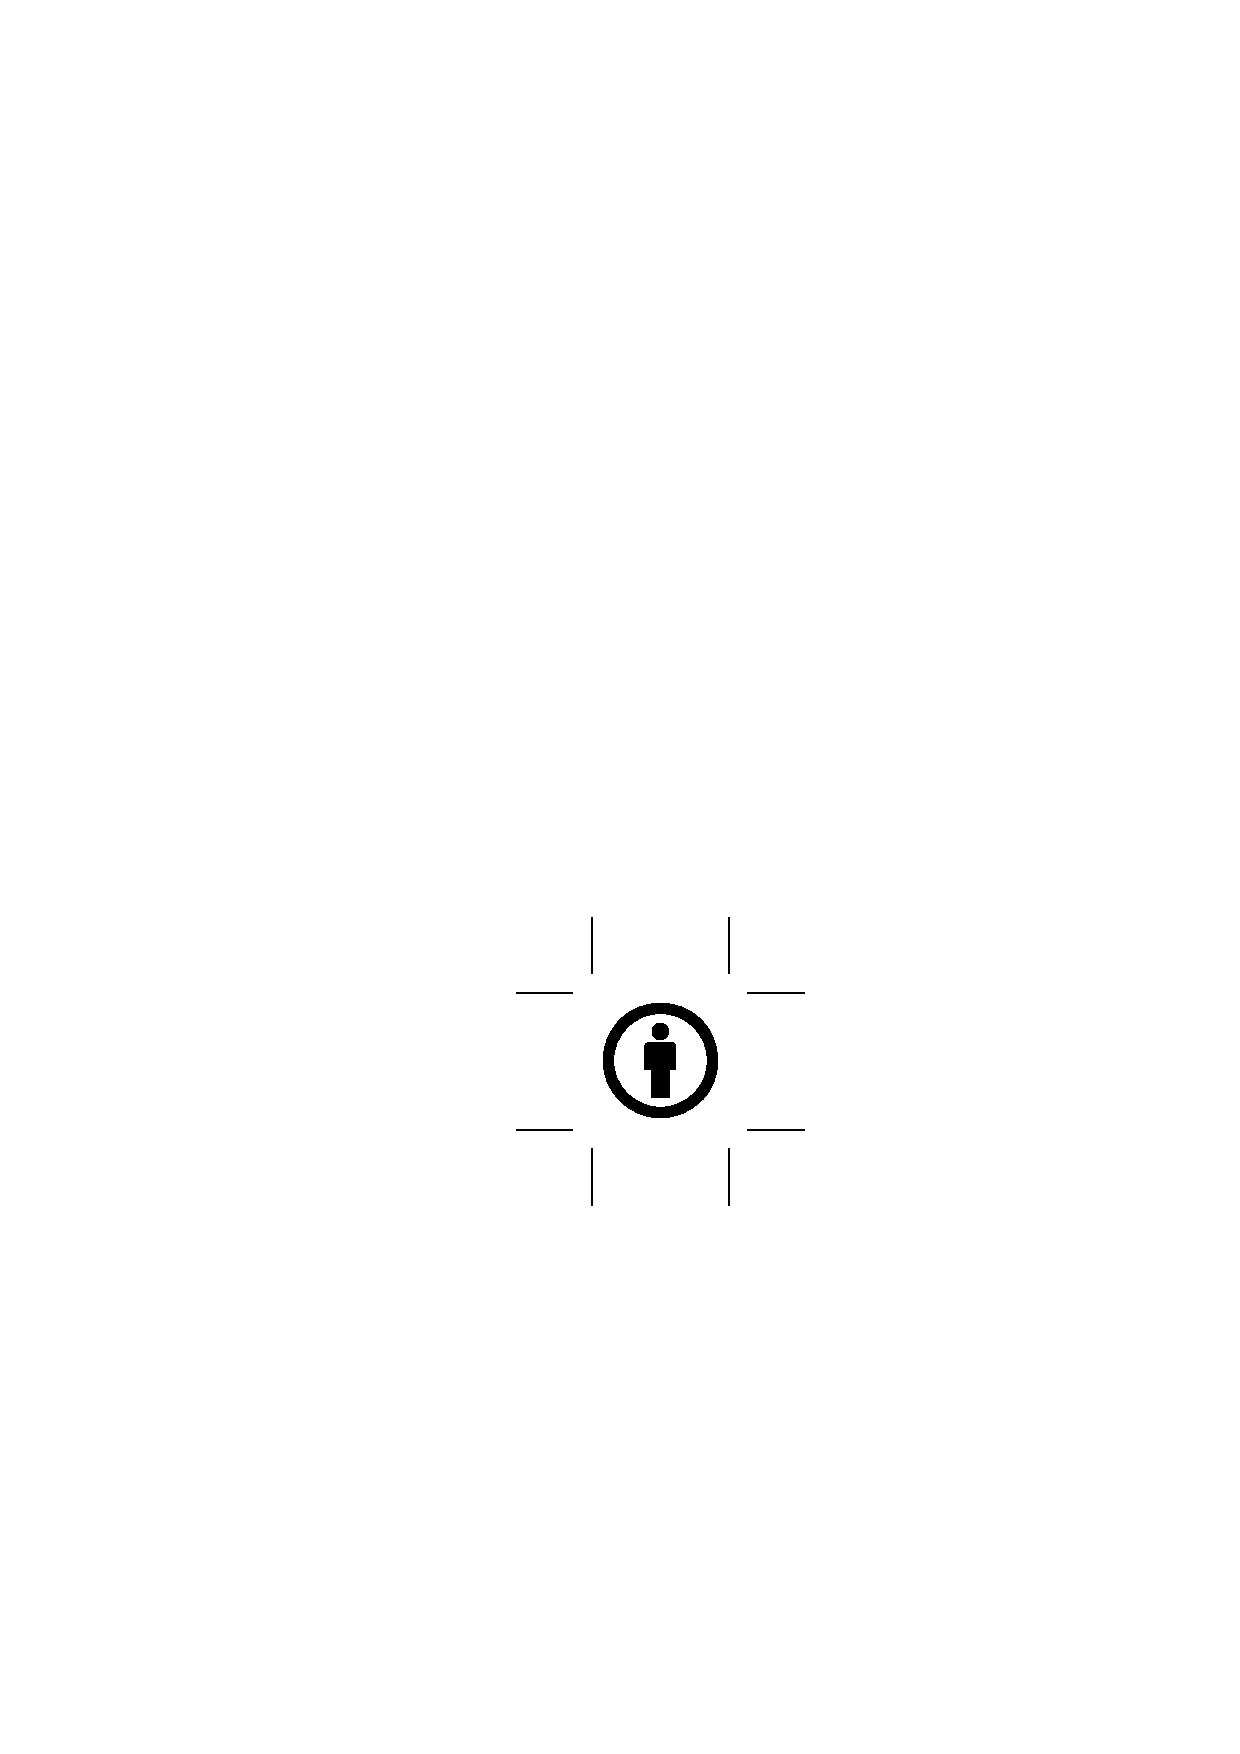
\includegraphics[height=4ex]{gfx/logos/creativecommons/by}

\smallskip

\noindent%
Veröffentlicht unter \emph{CC BY-SA 4.0 International}
\emph{(Namensnennung)} \\
\url{https://creativecommons.org/licenses/by/4.0/deed.de}

\end{otherlanguage}

\smallskip

\noindent%
Licensed under \emph{CC BY-SA 4.0 International}
\emph{(Attribution)} \\
\url{https://creativecommons.org/licenses/by/4.0/deed.en}

	\cleardoublepage% !TeX root = ../Thesis.tex

%*******************************************************
% Dedication
%*******************************************************
\thispagestyle{empty}
\phantomsection
\pdfbookmark[0]{Dedication}{Dedication}

\vspace*{3cm}

\begin{center}
    \emph{Ohana} means family. \\
    Family means nobody gets left behind, or forgotten. \\ \medskip
    --- Lilo \& Stitch
\end{center}

\medskip

\begin{center}
    Dedicated to the loving memory of Rudolf Miede. \\ \smallskip
    1939\,--\,2005
\end{center}

}{
	% !TeX root = ../Thesis.tex

%*******************************************************
% Titlepage
%*******************************************************
\pdfbookmark[0]{Cover}{cover}
\begin{titlepage}
    %\pdfbookmark[1]{\myTitle{}}{titlepage}
    % if you want the titlepage to be centered, uncomment and fine-tune the line below (KOMA classes environment)
    \begin{addmargin}[-1cm]{\iftoggle{adrianstyle}{-2cm}{-3cm}}
    \begin{center}
        \large

        
\includegraphics[width=6cm]{gfx/logos/tud_logo_rgb}
        
        \vfill

        \begingroup
            \color{CTtitle}\spacedallcaps{\myTitle{}} \\ \bigskip
        \endgroup

        \vspace{2ex}

        \spacedlowsmallcaps{\myName{}}

        \vfill

        \myDegree{}

        \vspace{2ex}

        \myTime{}

        \vfill

        \myDepartment{} \\
        \myFaculty{} \\
        \myUni{}

        \vfill

        
\includegraphics[width=5cm]{gfx/logos/seemoo_logo_rgb}
    \end{center}
    \end{addmargin}
\end{titlepage}

	% !TeX root = ../Thesis.tex

\thispagestyle{empty}

\ \vfill

\noindent%
\myName{}, \emph{\myTitle{}}, \myDegree, \myUni{}, \myYearPublication{}.

\bigskip

\noindent\myThesiscode{} \\
Date of submission: \myTime{}

\bigskip

\noindent\begin{tabular}{@{}l@{~}l@{}}
Advisor: & \myProf{} \\
Supervisor: & \mySupervisor{} \\
\end{tabular}

\bigskip

\noindent%
\myDepartment{} \\
\myFaculty{} \\
\myUni{}

% \bigskip

% \noindent%
% 
\includegraphics[height=4ex]{gfx/logos/creativecommons/cc}
% 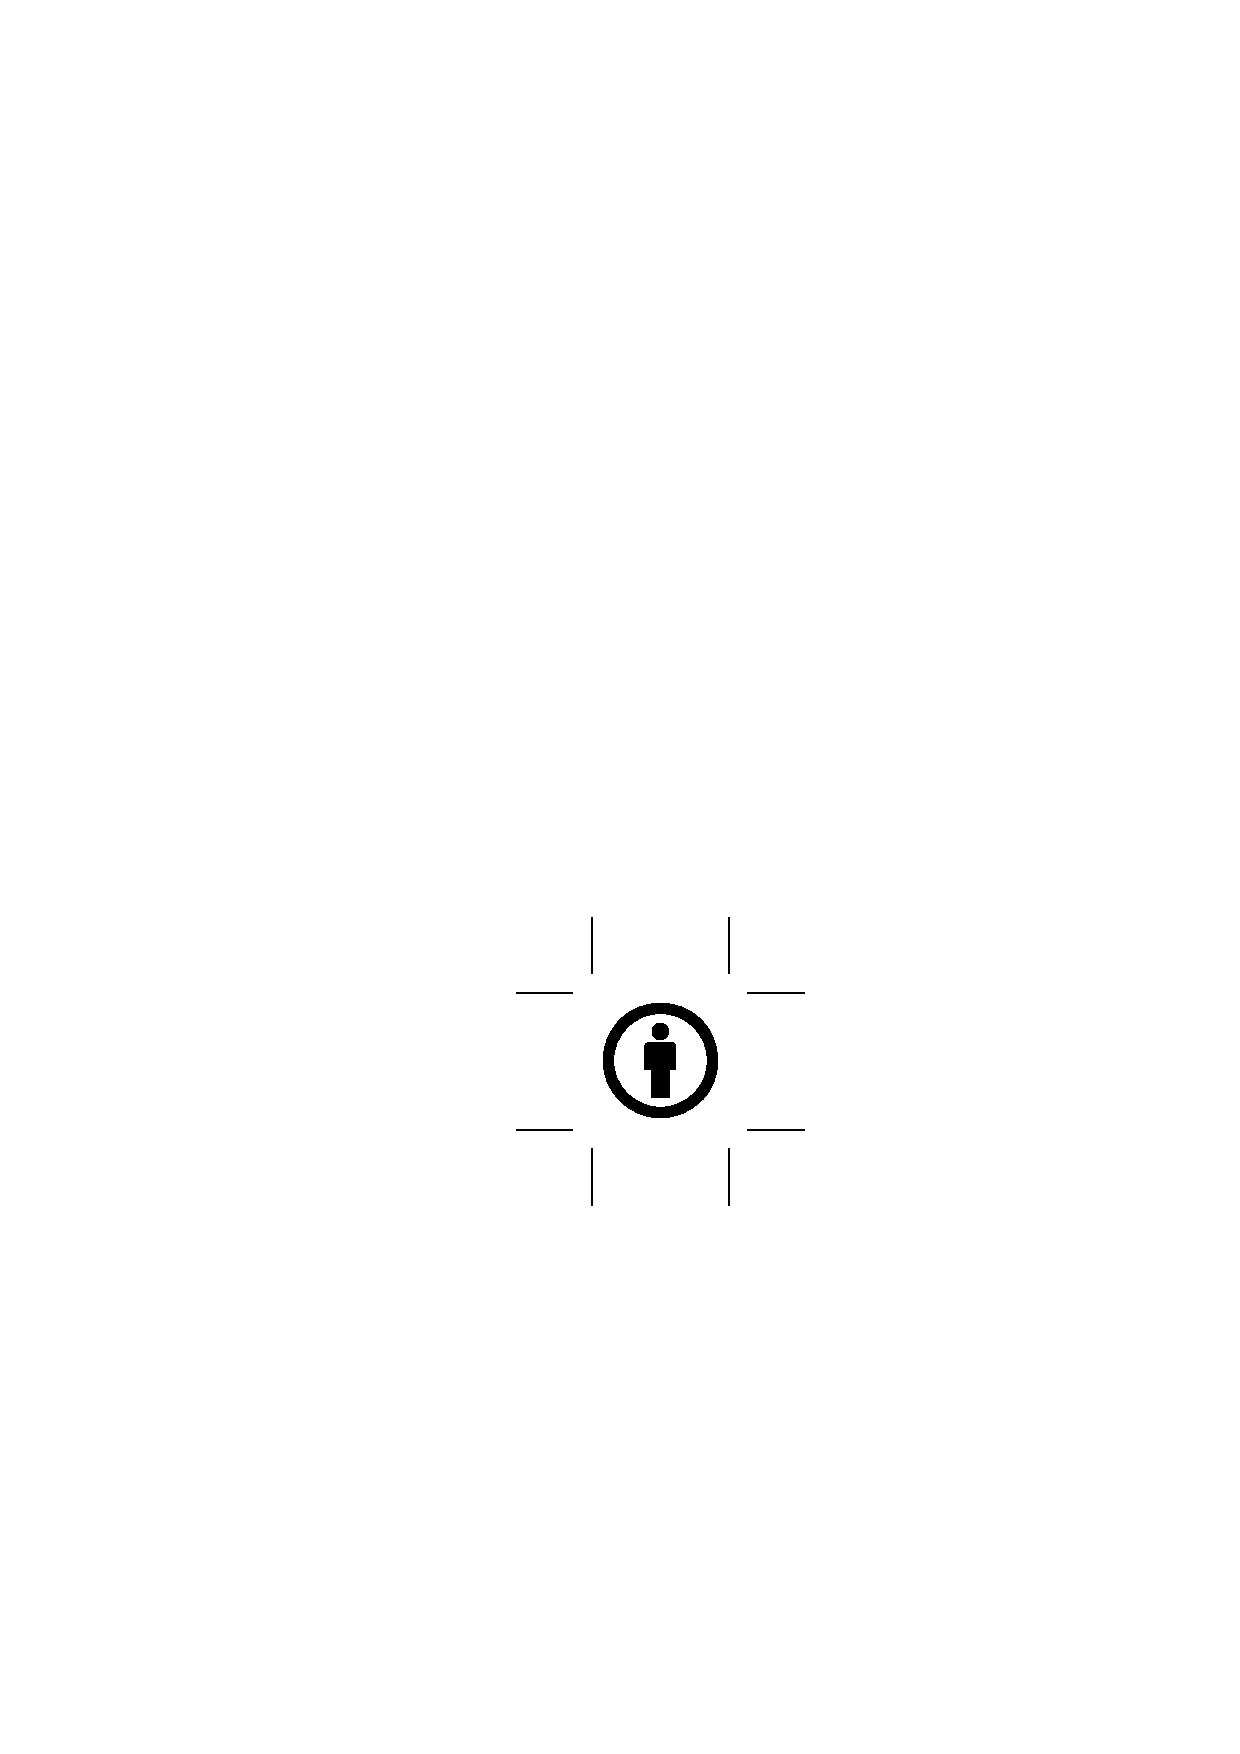
\includegraphics[height=4ex]{gfx/logos/creativecommons/by}

% \smallskip

% \begin{otherlanguage}{ngerman}

% \noindent%
% Veröffentlicht unter \emph{CC BY-SA 4.0 International}
% \emph{(Namensnennung)} \\
% \url{https://creativecommons.org/licenses/by/4.0/deed.de}

% \end{otherlanguage}

% \smallskip

% \noindent%
% Licensed under \emph{CC BY-SA 4.0 International}
% \emph{(Attribution)} \\
% \url{https://creativecommons.org/licenses/by/4.0/deed.en}
	
}
%\cleardoublepage\include{FrontBackmatter/Foreword}
\cleardoublepage% !TeX root = ../Thesis.tex

%*******************************************************
% Abstract
%*******************************************************
%\renewcommand{\abstractname}{Abstract}
\pdfbookmark[0]{Abstract}{Abstract}
% \addcontentsline{toc}{chapter}{\tocEntry{Abstract}}
\begingroup
\let\clearpage\relax
\let\cleardoublepage\relax
\let\cleardoublepage\relax

\chapter*{Abstract}
Short summary of the contents in English\dots a great guide by
Kent Beck how to write good abstracts can be found here:
\begin{center}
\url{https://plg.uwaterloo.ca/~migod/research/beckOOPSLA.html}
\end{center}

\vfill

\begin{otherlanguage}{ngerman}
\pdfbookmark[0]{Zusammenfassung}{Zusammenfassung}
\chapter*{Zusammenfassung}
Kurze Zusammenfassung des Inhaltes in deutscher Sprache\dots
\end{otherlanguage}

\endgroup

\vfill

\cleardoublepage% !TeX root = ../Thesis.tex

%*******************************************************
% Acknowledgments
%*******************************************************
\pdfbookmark[0]{Acknowledgments}{acknowledgments}

%\begin{flushright}{\slshape    
%    We have seen that computer programming is an art, \\ 
%    because it applies accumulated knowledge to the world, \\ 
%    because it requires skill and ingenuity, and especially \\
%    because it produces objects of beauty.} \\ \medskip
%    --- \defcitealias{knuth:1974}{Donald E. Knuth}%\citetalias{knuth:1974} \citep{knuth:1974}
%\end{flushright}



\bigskip

\begingroup
\let\clearpage\relax
\let\cleardoublepage\relax
\let\cleardoublepage\relax
\chapter*{Acknowledgments}
{\slshape 
I would like to express my deepest gratitude to my parents and my family for supporting me in all the years of my studies and also while writing this thesis.

\bigskip

Special thanks for giving helpful advice while writing this thesis goes to Prof. Matthias Hollick and Adrian Loch.

\bigskip

Furthermore, I especially thank Sandrine Adéla\"ide and Adrian Loch for proofreading my thesis.
}

\endgroup

\cleardoublepage% !TeX root = ../Thesis.tex

%*******************************************************
% Table of Contents
%*******************************************************
\pagestyle{scrheadings}
%\phantomsection
\pdfbookmark[0]{\contentsname}{tableofcontents}
\setcounter{tocdepth}{2} % <-- 2 includes up to subsections in the ToC
\setcounter{secnumdepth}{3} % <-- 3 numbers up to subsubsections
\manualmark
\markboth{\spacedlowsmallcaps{\contentsname}}{\spacedlowsmallcaps{\contentsname}}
\tableofcontents
\automark[section]{chapter}
\renewcommand{\chaptermark}[1]{\markboth{\spacedlowsmallcaps{#1}}{\spacedlowsmallcaps{#1}}}
\renewcommand{\sectionmark}[1]{\markright{\textsc{\thesection}\enspace\spacedlowsmallcaps{#1}}}
%*******************************************************
% List of Figures and of the Tables
%*******************************************************
\clearpage
% \pagestyle{empty} % Uncomment this line if your lists should not have any headlines with section name and page number
\begingroup
    \let\clearpage\relax
    \let\cleardoublepage\relax
    %*******************************************************
    % List of Figures
    %*******************************************************
    %\phantomsection
    %\addcontentsline{toc}{chapter}{\listfigurename}
    \pdfbookmark[0]{\listfigurename}{lof}
    \listoffigures

    \vspace{8ex}

    %*******************************************************
    % List of Tables
    %*******************************************************
    %\phantomsection
    %\addcontentsline{toc}{chapter}{\listtablename}
    \pdfbookmark[0]{\listtablename}{lot}
    \listoftables

    \vspace{8ex}
    % \newpage

    %*******************************************************
    % List of Listings
    %*******************************************************
    %\phantomsection
    %\addcontentsline{toc}{chapter}{\lstlistlistingname}
    \pdfbookmark[0]{\lstlistlistingname}{lol}
    \lstlistoflistings

    \vspace{8ex}

    %*******************************************************
    % Acronyms
    %*******************************************************
    %\phantomsection
    \pdfbookmark[0]{Acronyms}{acronyms}
    \printglossary[type=\acronymtype]

\endgroup
\iftoggle{phd}{
	\begin{refsection}[own] % use numbering of list of publications
	\cleardoublepage% !TeX root = ../Thesis.tex

%*******************************************************
% Publications
%*******************************************************
\chapterExtra{List of Publications}
\label{ch:AuthorPublications}

During the course of writing this thesis, I co-authored several papers and articles that I list below.

\nocite{*} % print all references


\section*{Journal and Magazine Articles}

{\small\printbibliography[heading=none,type=article,notkeyword=underreview]}


\section*{Conference and Workshop Papers}

{\small\printbibliography[heading=none,type=inproceedings,notkeyword=underreview,notkeyword=posterdemo]}


\section*{Posters and Demonstrators}

{\small\printbibliography[heading=none,type=inproceedings,notkeyword=underreview,keyword=posterdemo]}


\section*{Under Peer Review}

{\small\printbibliography[heading=none,type=article,keyword=underreview]}


\label{ch:AuthorPublicationsEnd}

	\cleardoublepage% !TeX root = ../Thesis.tex

%*******************************************************
\chapterExtra{Collaborations and My Contribution}
%*******************************************************
\label{ch:Collaborations}

% From Daniel Steinmetzer's dissertation
Systematically investigating a technical research topic and engineering the required tools is a demanding and interdisciplinary process. Most achievements could never evolve without collaborations in which colleagues and international partners integrated their intellectual forces. When working in teams, accounting particular contributions and components of the resulting publications to individual collaborators becomes almost impossible. This situation also applies to several contents of this thesis, which arise from collaborations, thus, cover joint contributions. Many of these collaborations persisted even longer than the research projects and became a long-term strategic partnership.
In our previous publications, all authors contributed by discussing ideas and debating on results throughout the whole project duration. Each of them has particular strengths that sometimes appear invisible. For this reason, I explicitly state and acknowledge---where possible---the contributions of my collaborators in the following.

% From Milan Stute's dissertation
In the following, I detail the contributions of my co-authors and myself per chapter. In addition, I follow the regulations of the \myFaculty{} at \myUni{} and give an account of the parts that include verbatim or revised fragments of previous publications that form this thesis as indicated in the preceding list of publications.\footnote{References in this chapter refer to my list of publications given on \cpagerefrange*{ch:AuthorPublications}{ch:AuthorPublicationsEnd}.}

\sloppy

\Cref{ch:introduction,ch:relatedwork} collate the contributions, background, and related work sections of the core papers that form this thesis~\cite{Stute2018a,Stute2020}.

% etc etc etc

\fussy

\label{ch:CollaborationsEnd}
	\end{refsection}
}{}
%********************************************************************
% Mainmatter
%*******************************************************
\addtocounter{table}{-1} % otherwise starts counting from 2
\cleardoublepage
\pagestyle{scrheadings}
\pagenumbering{arabic}
%\setcounter{page}{90}
% use \cleardoublepage here to avoid problems with pdfbookmark
\cleardoublepage
\iftoggle{parts}{
	\ctparttext{The first chapter of this part gives an introduction and a motivation to this thesis, followed by a presentation of related work found in the area of physical layer security. In the third chapter, we present some definitions and background information to make it easier for the reader to quickly understand the subsequent parts of this thesis.}
	\part{Introduction}
}{}
% !TeX root = ../Thesis.tex

%************************************************
\chapter{Introduction}\label{ch:introduction}
%************************************************
\glsresetall % Resets all acronyms to not used

Start a chapter with text and not with a section header. Open the
\emph{classicthesis-config.tex} file to insert the title of your thesis, the
names of your supervisors and the hand-in date of your thesis.

\section{First Section}
\label{sec:first_section}

After a section there should always be text before the next section. The first
paragraph is always without indentation. Starting from the second paragraph,
there is an indentation.

Here is an equation without numbers for referencing:
\begin{align*}
\underbrace{\begin{pmatrix}\mathcal{B}_1\\\mathcal{B}_2\\\vdots\\\mathcal{B}_R\end{pmatrix}}_\mathcal{B} &= \underbrace{\begin{pmatrix}H_{1,1} & H_{1,2} & \hdots & H_{1,T}\\H_{2,1} & H_{2,2} & \hdots & H_{2,T}\\\vdots & \vdots & \ddots & \vdots\\H_{R,1} & H_{R,2} & \hdots & H_{R,T}\end{pmatrix}}_{H_{A\rightarrow B}}\cdot \underbrace{\begin{pmatrix}\mathcal{A}_1\\\mathcal{A}_2\\\vdots\\\mathcal{A}_T\end{pmatrix}}_\mathcal{A}
\end{align*}

Here is an equation that you can reference:
\begin{align}
\underbrace{\begin{pmatrix}\mathcal{B}_1\\\mathcal{B}_2\\\vdots\\\mathcal{B}_R\end{pmatrix}}_\mathcal{B} &= \underbrace{\begin{pmatrix}H_{1,1} & H_{1,2} & \hdots & H_{1,T}\\H_{2,1} & H_{2,2} & \hdots & H_{2,T}\\\vdots & \vdots & \ddots & \vdots\\H_{R,1} & H_{R,2} & \hdots & H_{R,T}\end{pmatrix}}_{H_{A\rightarrow B}}\cdot \underbrace{\begin{pmatrix}\mathcal{A}_1\\\mathcal{A}_2\\\vdots\\\mathcal{A}_T\end{pmatrix}}_\mathcal{A}\label{eqn:example}
\end{align}

\subsection{Referencing}

Take a look in the following list to reference sections, figures and equations:
\begin{itemize}
  \item \Cref{sec:first_section}
  \item \Cref{fig:wiretapchannel}
  \item \Cref{eqn:example}
\end{itemize}

\subsection{Acronyms}
For acronyms you should use the \emph{glossaries} package and put your acronyms
in the \emph{FrontBackmatter/acronyms.tex} file. The first acronym is always
written in it's long form, the following occurrences are abbreviated: first
occurrence \gls{SNR}, second occurrence \gls{SNR}, plural \glspl{SNR}.

\subsection{Examples on Figures}

\sloppy
When using figures, use vector graphics whenever possible. In
\cref{fig:wiretapchannel,fig:example} are some examples to
generate vector graphics directly from \LaTeX code. The second example is based
on the \emph{matlab2tikz} script for matlab. You find an example in the
\mbox{\emph{gfx/matlab/create\_example\_graph.m}} file. TikZ is used to generate
the graphics. As it takes some time and memory to recompile a graphic, pdflatex
caches generated figures when the \lstinline|--enable-write18| switch is set
when calling \lstinline|pdflatex|. Graphics are only recompiled when you
uncomment the \lstinline|\tikzset{external/remake next}| command. Figures should
always appear after the first reference in the text or at the top of the same
page as the reference, but never before the reference. Prefer placing figures on
separate pages. Try to always have figures and text on each page. Or place
enough figures to fill a page only with figures.

\begin{figure}
\centering
\begin{tikzpicture}[node distance=6mm]
\node[dspsquare,minimum height=3.2em, minimum width=5em,text height=1em, fill=white]
		(source) {Source};
\node[dspsquare,minimum height=3.2em, minimum width=5em,text height=1em, fill=white, right=of source]
		(encoder) {Encoder};
\node[dspsquare,minimum height=3.2em, minimum width=7em,text height=2em, fill=white, right=of encoder]
		(mainch) {Main Channel\\$Q_M$};
\node[dspnodefull, right=of mainch] (n1) {};
\node[dspsquare,minimum height=3.2em, minimum width=5em,text height=1em, fill=white, right=of n1]
		(decoder) {Decoder};
\node[coordinate,right=of decoder] (n2) {};
\node[dspsquare,minimum height=3.2em, minimum width=10em,text height=2em, fill=white, below=1cm of n1]
		(wiretapch) {Wiretap Channel\\$Q_W$};
\node[coordinate,below=of wiretapch] (n3) {};

\draw[dspconn] (source) -- node[midway,above] {$S^K$} (encoder);
\draw[dspconn] (encoder) -- node[midway,above] {$X^N$} (mainch);
\draw[dspconn] (mainch) -- node[midway,above] {$Y^N$} (decoder);
\draw[dspconn] (decoder) -- node[midway,above] {$S^K$} (n2);
\draw[dspconn] (n1) -- (wiretapch);
\draw[dspconn] (wiretapch) -- (n3) node[below] {$Z^N$};
\end{tikzpicture}
\caption[The wiretap channel]{The wiretap channel (source: \cite{1975:Wyner})}
\label{fig:wiretapchannel}
\end{figure}

\subsection{Examples on Tables}

You can find an example table in \cref{tab:disasters} using the \emph{tabular} environment. Note the use of horizontal lines from the \emph{booktabs} package (\lstinline|\toprule|, \lstinline|\midrule|, and \lstinline|\bottomrule|) and removed whitespace at both sides of the table (\lstinline|@{}|) as proposed by Markus Püschel.\footnote{\url{https://www.inf.ethz.ch/personal/markusp/teaching/guides/guide-tables.pdf}}

\begin{table}
\centering
\begin{tabular}{@{} lclr @{}} % @{} removes white spaces
	\toprule
	\tableheadline{Disaster} & \tableheadline{Year} & \tableheadline{Country} & \tableheadline{Area (km\textsuperscript{2})} \\
	\midrule
	Nepal earthquake & 2015 & Nepal & 3\,610 \\
	Cyclone Pam & 2015 & Vanuatu & 12\,190 \\
	Ludian earthquake & 2014 & China & 1\,487 \\
	Typhoon Haiyan & 2013 & Philippines & 71\,503 \\
	Christchurch earthquake & 2011 & New Zealand & 1\,426 \\
	East Africa drought & 2011 & East Africa & 2\,346\,466 \\
	Tropical storm Washi & 2011 & Philippines & 104\,530 \\
	Tohoku earthquake & 2011 & Japan & 83\,955 \\
	Haiti earthquake & 2010 & Haiti & 27\,750 \\
	Afghanistan blizzard & 2008 & Afghanistan & 652\,864 \\
	Sichuan earthquake & 2008 & China & 485\,000 \\
	Cyclone Nargis & 2008 & Myanmar & 676\,578 \\
	\bottomrule
\end{tabular}
% Use alternative short title for table of contents
\caption[Large-scale natural disasters]{Large-scale natural disasters in the last ten years}
\label{tab:disasters}
\end{table}

\section{Margin Notes}

Especially in the standard SEEMOO template with wide margins, you are
\marginpar{Here you can add text to the margin. For example, to
summarize the section next to it.} encouraged to insert text into the
margins. If you decide to do so, plan to have at least one margin note
per double page.

\section{Some Example Text}
\lipsum[3]

\begin{figure}
\centering
\setlength\figureheight{5cm}
\setlength\figurewidth{0.86\textwidth}
% uncomment the following line to recompile the figure when it changes otherwise a cached version is used
%\tikzset{external/remake next}
% This file was created by matlab2tikz v0.4.7 running on MATLAB 8.1.
% Copyright (c) 2008--2014, Nico Schlmer <nico.schloemer@gmail.com>
% All rights reserved.
% Minimal pgfplots version: 1.3
% 
% The latest updates can be retrieved from
%   http://www.mathworks.com/matlabcentral/fileexchange/22022-matlab2tikz
% where you can also make suggestions and rate matlab2tikz.
% 
\begin{tikzpicture}[%
font=\footnotesize
]

\begin{axis}[%
width=\figurewidth,
height=\figureheight,
scale only axis,
xmin=1,
xmax=100,
xlabel={x axis},
ymin=-1.5,
ymax=1.5,
ylabel={y axis},
legend style={draw=black,fill=white,legend cell align=left},
clip mode=individual,transpose legend,legend columns=2,legend style={at={(0,1)},anchor=north west,draw=black,fill=white,legend cell align=left}
]
\addplot [color=blue,solid]
  table[row sep=crcr]{1	0.309016994374947\\
2	0.587785252292473\\
3	0.809016994374947\\
4	0.951056516295154\\
5	1\\
6	0.951056516295154\\
7	0.809016994374947\\
8	0.587785252292473\\
9	0.309016994374948\\
10	1.22464679914735e-16\\
11	-0.309016994374947\\
12	-0.587785252292473\\
13	-0.809016994374947\\
14	-0.951056516295154\\
15	-1\\
16	-0.951056516295154\\
17	-0.809016994374948\\
18	-0.587785252292473\\
19	-0.309016994374948\\
20	-2.44929359829471e-16\\
21	0.309016994374947\\
22	0.587785252292472\\
23	0.809016994374947\\
24	0.951056516295154\\
25	1\\
26	0.951056516295154\\
27	0.809016994374948\\
28	0.587785252292473\\
29	0.309016994374948\\
30	3.67394039744206e-16\\
31	-0.309016994374947\\
32	-0.587785252292473\\
33	-0.809016994374947\\
34	-0.951056516295153\\
35	-1\\
36	-0.951056516295154\\
37	-0.809016994374948\\
38	-0.587785252292473\\
39	-0.309016994374948\\
40	-4.89858719658941e-16\\
41	0.309016994374945\\
42	0.587785252292473\\
43	0.809016994374947\\
44	0.951056516295153\\
45	1\\
46	0.951056516295154\\
47	0.809016994374947\\
48	0.587785252292474\\
49	0.30901699437495\\
50	6.12323399573677e-16\\
51	-0.309016994374945\\
52	-0.587785252292473\\
53	-0.809016994374948\\
54	-0.951056516295153\\
55	-1\\
56	-0.951056516295154\\
57	-0.809016994374949\\
58	-0.587785252292474\\
59	-0.30901699437495\\
60	-7.34788079488412e-16\\
61	0.309016994374948\\
62	0.587785252292472\\
63	0.809016994374948\\
64	0.951056516295153\\
65	1\\
66	0.951056516295154\\
67	0.809016994374949\\
68	0.587785252292474\\
69	0.309016994374947\\
70	8.57252759403147e-16\\
71	-0.309016994374948\\
72	-0.587785252292472\\
73	-0.809016994374946\\
74	-0.951056516295153\\
75	-1\\
76	-0.951056516295154\\
77	-0.809016994374947\\
78	-0.587785252292474\\
79	-0.309016994374947\\
80	-9.79717439317883e-16\\
81	0.309016994374945\\
82	0.587785252292469\\
83	0.809016994374948\\
84	0.951056516295153\\
85	1\\
86	0.951056516295154\\
87	0.809016994374949\\
88	0.587785252292477\\
89	0.309016994374947\\
90	1.10218211923262e-15\\
91	-0.309016994374945\\
92	-0.587785252292472\\
93	-0.809016994374946\\
94	-0.951056516295154\\
95	-1\\
96	-0.951056516295154\\
97	-0.809016994374949\\
98	-0.587785252292477\\
99	-0.309016994374947\\
100	-1.22464679914735e-15\\
};
\addlegendentry{sinus};

\end{axis}
\end{tikzpicture}%
\caption[Caption for list of figures]{Caption of figure}
\label{fig:example}
\end{figure}

\lipsum[6-10]

% !TeX root = ../Thesis.tex

%*****************************************
\chapter{Related Work}\label{ch:relatedwork}
%*****************************************
\glsresetall % Resets all acronyms to not used

\lipsum[4]

\iftoggle{parts}{
	\cleardoublepage
	\ctparttext{The contribution starts with a design chapter, where we mathematically describe the design of the physical layer security system, as well as the adaptive filter of the attacker. After the design follows the implementation on WARP nodes. Here we give an insight into the challenges of implementing the designed MIMO communication system. The last chapter concentrates on evaluating the performance of our proposed attack in simulation and practice.}
	\part{Contribution}
}{}
% !TeX root = ../Thesis.tex

%************************************************
\chapter{Design}\label{ch:design}
%************************************************
\glsresetall % Resets all acronyms to not used

\lipsum[9]

% !TeX root = ../Thesis.tex

%************************************************
\chapter{Implementation}\label{ch:implementation}
%************************************************
\glsresetall % Resets all acronyms to not used

\lipsum[4]

% !TeX root = ../Thesis.tex

%************************************************
\chapter{Evaluation}\label{ch:evaluation}
%************************************************
\glsresetall % Resets all acronyms to not used

\lipsum[5]

\iftoggle{parts}{
	\cleardoublepage
	\ctparttext{After the evaluation, we further discuss the results and give an outlook. In addition, we finish this work with conclusions.}
	\part{Discussion and Conclusions}
}{}
% !TeX root = ../Thesis.tex

%************************************************
\chapter{Discussion}\label{ch:Discussion} % $\mathbb{ZNR}$
%************************************************
\glsresetall % Resets all acronyms to not used

\lipsum[6]

% !TeX root = ../Thesis.tex

%************************************************
\chapter{Conclusions}\label{ch:Conclusions}
%************************************************
\glsresetall % Resets all acronyms to not used

\lipsum[7]

% ********************************************************************
% Backmatter
%*******************************************************
\iftoggle{parts}{}{
	\addtocontents{toc}{\protect\vspace{\beforebibskip}} % add space between main chapters and appendix if we do not use parts
}
\appendix
%\renewcommand{\thechapter}{\alph{chapter}}
\cleardoublepage
\iftoggle{parts}{
	\part{Appendix}
}{}
% !TeX root = ../Thesis.tex

%********************************************************************
% Some Proof (Appendix)
%*******************************************************
% If problems with the headers: get headings in appendix etc. right
%\markboth{\spacedlowsmallcaps{Appendix}}{\spacedlowsmallcaps{Appendix}}
\chapter{Some Proof}\label{ch:SomeProof}
\glsresetall % Resets all acronyms to not used

\lipsum[8]

%********************************************************************
% Other Stuff in the Back
%*******************************************************
\iftoggle{parts}{
	% !TeX root = ../Thesis.tex

\pdfbookmark[-1]{Back Matter}{backmatter}

}{}
\cleardoublepage% !TeX root = ../Thesis.tex

%********************************************************************
% Bibliography
%*******************************************************
% work-around to have small caps also here in the headline
% https://tex.stackexchange.com/questions/188126/wrong-header-in-bibliography-classicthesis
% Thanks to Enrico Gregorio
\defbibheading{bibintoc}[\bibname]{%
  \phantomsection
  \manualmark
  \markboth{\spacedlowsmallcaps{#1}}{\spacedlowsmallcaps{#1}}%
  \addtocontents{toc}{\protect\vspace{\beforebibskip}}%
  \addcontentsline{toc}{chapter}{\tocEntry{#1}}%
  \chapter*{#1}%
}
\printbibliography[heading=bibintoc]

% Old version, will be removed later
% work-around to have small caps also here in the headline
%\manualmark
%\markboth{\spacedlowsmallcaps{\bibname}}{\spacedlowsmallcaps{\bibname}} % work-around to have small caps also
%\phantomsection
%\refstepcounter{dummy}
%\addtocontents{toc}{\protect\vspace{\beforebibskip}} % to have the bib a bit from the rest in the toc
%\addcontentsline{toc}{chapter}{\tocEntry{\bibname}}
%\label{app:bibliography}
%\printbibliography

\iftoggle{phd}{
	%\cleardoublepage% !TeX root = ../Thesis.tex

%************************************************
\chapterExtra{Curriculum Vit\ae}\label{ch:CurriculumVitae}
%************************************************

\begin{cv}{}

\renewcommand*{\cvlistheadingfont}{\spacedlowsmallcaps} % same as sections
\renewcommand*{\cvlabelfont}{\itshape}
\setlength\cvlabelwidth{60pt}

\begin{cvlist}{{Personal Information}}
    \item[Name] \myName
    \item[Date of Birth] \myBirthDate
    \item[Place of Birth] \myBirthPlace
    \item[Nationality] \myNationality
\end{cvlist}


\begin{cvlist}{{Education}}

\item[since 2018] \textbf{Doctoral Candidate} \\
Computer Science, Technische Universiät Darmstadt, Darmstadt, Germany

\item[2016--2018] \textbf{Master of Science} \\
Computer Science, Technische Universität Darmstadt, Darmstadt, Germany

\item[2013--2016] \textbf{Bachelor of Science} \\
Computer Science, Technische Universität Darmstadt, Darmstadt, Germany

\end{cvlist}


\begin{cvlist}{{Work Experience}}

\item[since 2012] \textbf{Research Associate} \\
Secure Mobile Networking Lab, Technische Universität Darmstadt, Darmstadt, Germany.

\end{cvlist}


\begin{cvlist}{{Awards}}

\item[Publication] \textbf{Best Community Paper Award at ACM MobiCom '18} \\
Paper: \enquote{One Billion Apples’ Secret Sauce: Recipe for the Apple Wireless Direct Link Ad hoc Protocol}.

\end{cvlist}        


\begin{cvlist}{{Supervised Student Theses}}

\item[B.\,Sc. Thesis] \textbf{Another Student}, \enquote{A Very Cool Topic}, 2018.

\item[M.\,Sc. Thesis] \textbf{Milan Schmittner}, \enquote{Scalable and Secure Multicast Routing for Mobile Ad-hoc Networks}, 2014.

\end{cvlist}


% \begin{cvlist}{{Miscellaneous}}

% \item[Teaching] Organization of the integrated course \enquote{Network Security}.

% \end{cvlist}


\date{\myLocation{}, \myTime{}}

\end{cv}
 % not required in final submission
	\cleardoublepage%!TEX root = ../Thesis.tex

\begin{otherlanguage}{ngerman}

%*******************************************************
\chapterExtra{Erklärung zur Dissertationsschrift}
%*******************************************************

% Promotionsordnung und mehr des FB 20
% https://www.informatik.tu-darmstadt.de/forschung_fb20/wissenschaftliche_karriere/promotion/index.de.jsp

\begin{flushright}
    \emph{\small gemäß §\,9 der Allgemeinen Bestimmungen der Promotionsordnung der \\
    \myUni{} vom \formatdate{12}{1}{1990} (ABI. 1990, S.\,658) \\
    in der Fassung der 8.\,Novelle vom \formatdate{1}{3}{2018}}
\end{flushright}
Hiermit versichere ich, \myName{}, die vorliegende Dissertationsschrift ohne Hilfe Dritter und nur mit den angegebenen Quellen und Hilfsmitteln angefertigt zu haben. Alle Stellen, die Quellen entnommen wurden, sind als solche kenntlich gemacht worden. Eigenzitate aus vorausgehenden wissenschaftlichen Veröffentlichungen werden in Anlehnung an die Hinweise des Promotionsausschusses \myFacultyDE{} zum Thema \enquote{Eigenzitate in wissenschaftlichen Arbeiten} (EZ-2014/10) in Kapitel \enquote{\emph{Collaborations and My Contribution}} auf \cpagerefrange*{ch:Collaborations}{ch:CollaborationsEnd} gelistet. Diese Arbeit hat in gleicher oder ähnlicher Form noch keiner Prüfungsbehörde vorgelegen. In der abgegebenen Dissertationsschrift stimmen die schriftliche und die elektronische Fassung überein.
% cannot use \nameref for chapter name, see https://bitbucket.org/amiede/classicthesis/issues/170/nameref-for-chapter-showing-the-previous

\bigskip

\noindent\textit{\myLocation{}, \myTime{}}

\begin{flushright}
    \begin{tabular}{m{5cm}}
        \\ \hline
        \centering\myName{} \\
    \end{tabular}
\end{flushright}

\end{otherlanguage}

}{
	\cleardoublepage% !TeX root = ../Thesis.tex

%*******************************************************
% Declaration
%*******************************************************

% Text aus: https://www.intern.tu-darmstadt.de/media/dezernat_ii/referat_iig/formulare_vorlagen/pm_1/erklaerungen/Erklaerung_zur_Abschlussarbeit_Vorlage.docx
% Stand: 3. Juni 2019

\begingroup

\begin{otherlanguage}{ngerman}
\chapterExtra{Erklärung zur Abschlussarbeit}
\begin{flushright}
	\emph{gemäß §\,22 Abs.\,7 und §\,23 Abs.\,7 APB TU Darmstadt}
\end{flushright}
Hiermit versichere ich, \myName{}, die vorliegende \myDegree{} gemäß §\,22 Abs.\,7 APB der TU Darmstadt ohne Hilfe Dritter und nur mit den angegebenen Quellen und Hilfsmitteln angefertigt zu haben. Alle Stellen, die Quellen entnommen wurden, sind als solche kenntlich gemacht worden. Diese Arbeit hat in gleicher oder ähnlicher Form noch keiner Prüfungsbehörde vorgelegen.
Mir ist bekannt, dass im Falle eines Plagiats (§\,38 Abs.\,2 APB) ein Täuschungsversuch vorliegt, der dazu führt, dass die Arbeit mit 5,0 bewertet und damit ein Prüfungsversuch verbraucht wird. Abschlussarbeiten dürfen nur einmal wiederholt werden.
Bei der abgegebenen Thesis stimmen die schriftliche und die zur Archivierung eingereichte elektronische Fassung gemäß §\,23 Abs.\,7 APB überein.
\end{otherlanguage}

\vfill

\let\cleardoublepage\relax
\chapter*{Thesis Statement}
\begin{flushright}
	\emph{pursuant to §\,22 paragraph 7 and §\,23 paragraph 7 of APB TU Darmstadt}
\end{flushright}

I herewith formally declare that I, \myName{}, have written the submitted \myDegree{} independently pursuant to §\,22 paragraph 7 of APB TU Darmstadt. I did not use any outside support except for the quoted literature and other sources mentioned in the paper. I clearly marked and separately listed all of the literature and all of the other sources which I employed when producing this academic work, either literally or in content. This thesis has not been handed in or published before in the same or similar form.
I am aware, that in case of an attempt at deception based on plagiarism (§\,38 paragraph 2 APB), the thesis would be graded with 5.0 and counted as one failed examination attempt. The thesis may only be repeated once.
In the submitted thesis the written copies and the electronic version for archiving are pursuant to §\,23 paragraph 7 of APB identical in content.

\vfill

\noindent\textit{\myLocation{}, \myTime{}}

\begin{flushright}
    \begin{tabular}{m{5cm}}
        \\ \hline
        \centering\myName{} \\
    \end{tabular}
\end{flushright}

\endgroup

}
%\cleardoublepage% !TeX root = ../Thesis.tex

\pagestyle{empty}

\hfill

\vfill


\pdfbookmark[0]{Colophon}{colophon}
\section*{Colophon}
This document was typeset using the typographical look-and-feel \texttt{classicthesis} developed by Andr\'e Miede and Ivo Pletikosić.
The style was inspired by Robert Bringhurst's seminal book on typography ``\emph{The Elements of Typographic Style}''.
\texttt{classicthesis} is available for both \LaTeX\ and \mLyX:
\begin{center}
\url{https://bitbucket.org/amiede/classicthesis/}
\end{center}
Happy users of \texttt{classicthesis} usually send a real postcard to the author, a collection of postcards received so far is featured here:
\begin{center}
\url{http://postcards.miede.de/}
\end{center}
Thank you very much for your feedback and contribution.

\bigskip

\noindent\finalVersionString

%Hermann Zapf's \emph{Palatino} and \emph{Euler} type faces (Type~1 PostScript fonts \emph{URW
%Palladio L} and \emph{FPL}) are used. The ``typewriter'' text is typeset in \emph{Bera Mono},
%originally developed by Bitstream, Inc. as ``Bitstream Vera''. (Type~1 PostScript fonts were made
%available by Malte Rosenau and
%Ulrich Dirr.)

%\paragraph{note:} The custom size of the textblock was calculated
%using the directions given by Mr. Bringhurst (pages 26--29 and
%175/176). 10~pt Palatino needs  133.21~pt for the string
%``abcdefghijklmnopqrstuvwxyz''. This yields a good line length between
%24--26~pc (288--312~pt). Using a ``\emph{double square textblock}''
%with a 1:2 ratio this results in a textblock of 312:624~pt (which
%includes the headline in this design). A good alternative would be the
%``\emph{golden section textblock}'' with a ratio of 1:1.62, here
%312:505.44~pt. For comparison, \texttt{DIV9} of the \texttt{typearea}
%package results in a line length of 389~pt (32.4~pc), which is by far
%too long. However, this information will only be of interest for
%hardcore pseudo-typographers like me.%
%
%To make your own calculations, use the following commands and look up
%the corresponding lengths in the book:
%\begin{verbatim}
%    \settowidth{\abcd}{abcdefghijklmnopqrstuvwxyz}
%    \the\abcd\ % prints the value of the length
%\end{verbatim}
%Please see the file \texttt{classicthesis.sty} for some precalculated
%values for Palatino and Minion.
%
%    \settowidth{\abcd}{abcdefghijklmnopqrstuvwxyz}
%    \the\abcd\ % prints the value of the length

% ********************************************************************
% Game Over: Restore, Restart, or Quit?
%*******************************************************
\end{document}
% ********************************************************************
